\documentclass[11pt]{article}

\usepackage[margin=1in]{geometry}
\usepackage{booktabs}
\usepackage{tabularx}
\usepackage{array}
\usepackage{enumitem}
\usepackage{xcolor}
\usepackage{hyperref}
\usepackage{tikz}
\usetikzlibrary{arrows.meta,positioning,shapes.geometric}

\hypersetup{
  colorlinks=true,
  linkcolor=blue,
  citecolor=blue,
  urlcolor=blue
}

\title{Data Center Cooling Research Tools: A Curated, Refreshable Catalog From Thermal Mechanisms to Digital Twins}
\author{Repository Maintainers\\UARK-NED3\\\texttt{https://github.com/UARK-NED3/Data-Center-Cooling-Research-Tools}}
\date{July 20, 2026}

\begin{document}
\maketitle

\begin{abstract}
Data center cooling research now spans boiling and droplet diagnostics, chip and package thermal design, rack liquid loops, facility energy simulation, water and carbon accounting, control, digital twins, operations telemetry, and metadata. This breadth makes tool discovery difficult: repositories, standards, commercial workflows, and paper artifacts are scattered across different communities and are rarely labeled with the physical scale or evidence level needed by thermal-fluid researchers. This paper describes the \emph{Data Center Cooling Research Tools} repository, a curated and refreshable catalog organized around the cooling stack from mechanism-scale experiments to campus-scale operation. The repository combines a human-reviewed README catalog, a candidate-review workflow, generated CSV/SVG summaries with explicit validation-basis and run-status metadata, a catalog-quality report, a validation-review queue with review-age, candidate-review-state, and source-missing signals, a validation execution matrix that separates runnable smoke tests from blocked, hardware-in-loop, or manual evidence work, a validation runbook that states the minimum probe and evidence packet for queued rows, a validation next-actions report that ranks stale ready rows and blockers into a finite daily closure batch, a validation-debt report that ages stale ready items and blockers, a runtime prerequisite check for refresh environments, a weekly GitHub discovery script, and review logs that separate validated resources from educational examples, vendor material, and low-confidence candidates. The current catalog highlights several major trends: the movement of direct-to-chip liquid cooling toward open specifications, Redfish liquid-cooling schemas, and reference tools, the growth of Gymnasium/FMUs/Modelica/EnergyPlus-style control and facility-modeling workflows, safety-aware digital-twin deployment, semantic metadata and telemetry correlation for liquid-cooling operations, device-aware thermal setpoint optimization, synthetic-data PUE/control teaching artifacts, the expansion of facility metrics beyond PUE toward water-impact, heat-reuse, and grid-interactive accounting, and the need to keep mechanism-level diagnostics connected to system-level models. The contribution is not a new cooling model; it is an evidence-aware research map and maintenance workflow that helps researchers find tools, understand caveats, and keep the landscape current without turning search results into unsupported citations.
\end{abstract}

\noindent\textbf{Keywords:} data center cooling; liquid cooling; thermal management; digital twins; PUE; WUE; reinforcement learning; Modelica; EnergyPlus; research tools

\section{Introduction}

AI and high-performance computing loads have made data center cooling a multi-scale research problem. A single study may need chip-level heat spreading, cold-plate pressure drop, coolant distribution, facility HVAC, workload scheduling, and sustainability accounting. Standards and professional resources, including ASHRAE's data center guidance hub, TC 9.9 resources, ANSI/ASHRAE Standard 90.4-2025 listings, and the PNNL/ASHRAE/NEMA AI Data Center Energy Performance Framework, provide boundaries and planning context for thermal environments, energy design, water use, grid interaction, commissioning, operation, and retrofit decisions \cite{ASHRAEDataCenterResources2026,ASHRAEAIDCFramework2026}. Open Compute Project (OCP) cooling resources similarly reflect the increasing relevance of liquid cooling, cold plates, coolant distribution units, immersion, door heat exchangers, and heat reuse for high-density systems \cite{OCPCoolingEnvironments2026,OCPColdPlate2026}. DMTF's Redfish liquid-cooling equipment guidance adds operations-facing schema context for cooling distribution units, immersion systems, heat exchangers, facility cooling loops, coolant connectors, leak detection, pumps, reservoirs, thermal metrics, and Facility/ThermalEquipment resources \cite{DMTFRedfishLiquidCooling2025}. NVIDIA DSX documentation and NVIDIA's June 2026 liquid-cooling article are also useful current signals for high-temperature, fully liquid-cooled AI factory design, including DSX Sim, DSX Exchange, facilities reference designs, 45~$^\circ$C inlet context, and dry-cooler/chiller implications \cite{NVIDIADSX2026,NVIDIALiquidCooling2026}. Vendor and reference-design sources are treated as context rather than independent performance data. At the same time, research code and benchmark environments are appearing quickly in GitHub repositories, often before they have stable papers, long-term maintenance, or independent validation.

The resulting problem is not simply lack of tools. It is lack of a usable map. Researchers need to know whether a resource is a standard, a validated model, a paper artifact, a vendor reference, an educational example, or only a candidate discovered by search. They also need to see which physical scale a resource addresses. A Modelica facility model, a rack leak-monitoring reference implementation, an EnergyPlus workflow, a boiling-image segmentation codebase, and a reinforcement-learning cooling benchmark may all be relevant to data center cooling, but they answer different engineering questions and carry different evidence limits.

The \emph{Data Center Cooling Research Tools} repository was created as a curated hub for this landscape \cite{DCCRT2026}. It is intentionally breadth-first: the goal is not to promote one solver, one model, or one laboratory workflow, but to help researchers start in the right part of the cooling stack and then evaluate resources with explicit caveats. This paper documents the catalog structure, maintenance workflow, generated summaries, and current trend interpretation. The paper also describes why a living repository is useful for an area where research artifacts, open specifications, and control benchmarks are changing faster than conventional review articles can be updated.

\section{Repository Design}

\subsection{Scope}

The repository includes resources that help researchers design, model, test, monitor, optimize, benchmark, or evaluate data center cooling systems. Included entries may be open-source repositories, commercial tools, standards, datasets, benchmark environments, paper artifacts, vendor technical references, or practical workflows. Generic data center infrastructure is excluded unless the cooling, energy, telemetry, sustainability, control, or liquid-cooling hardware connection is explicit.

\subsection{Cooling-Stack Taxonomy}

The README catalog is organized by physical scale rather than by software genre. This makes the repository easier to use when a researcher begins with an engineering question, such as ``How should I model rack liquid loops?'' or ``Which tools connect cooling control to PUE and WUE?'' Figure~\ref{fig:taxonomy} shows the current taxonomy.

\begin{figure*}[t]
\centering
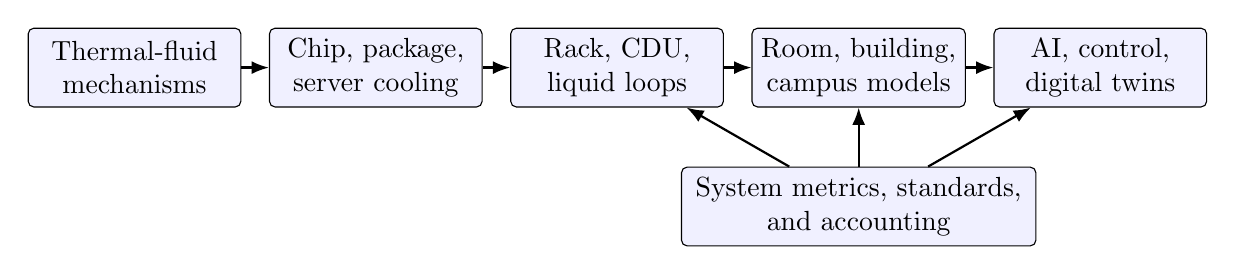
\begin{tikzpicture}[
  box/.style={draw, rounded corners=2pt, align=center, minimum width=2.7cm, minimum height=1.0cm, fill=blue!6},
  arrow/.style={-{Latex[length=2.2mm]}, thick}
]
\node[box] (mech) {Thermal-fluid\\mechanisms};
\node[box, right=0.35cm of mech] (chip) {Chip, package,\\server cooling};
\node[box, right=0.35cm of chip] (rack) {Rack, CDU,\\liquid loops};
\node[box, right=0.35cm of rack] (facility) {Room, building,\\campus models};
\node[box, right=0.35cm of facility] (ops) {AI, control,\\digital twins};
\node[box, below=0.75cm of facility, minimum width=4.5cm] (metrics) {System metrics, standards,\\and accounting};
\draw[arrow] (mech) -- (chip);
\draw[arrow] (chip) -- (rack);
\draw[arrow] (rack) -- (facility);
\draw[arrow] (facility) -- (ops);
\draw[arrow] (metrics) -- (rack);
\draw[arrow] (metrics) -- (facility);
\draw[arrow] (metrics) -- (ops);
\end{tikzpicture}
\caption{Cooling-stack taxonomy used by the repository. The taxonomy keeps mechanism-level evidence, hardware integration, facility modeling, operation, and system metrics connected while preserving their different assumptions and validation needs.}
\label{fig:taxonomy}
\end{figure*}

The taxonomy also helps avoid a common failure mode in tool lists: placing all AI, CFD, standards, and hardware references in one undifferentiated table. In the current repository, a tool is useful only when the entry identifies its scale, workflow, and evidence caveat.

\subsection{Evidence Labels And Caveats}

Every catalog row includes a compact note that states what the resource is useful for and how cautiously it should be interpreted. The contribution workflow uses labels such as include, candidate, adjacent, educational, and exclude. These labels are not journal-quality evidence grades, but they prevent search-derived repositories from being treated as validated engineering tools. For example, an educational reinforcement-learning project may be useful for teaching control structure but should not be cited as proof that a controller is safe for production cooling systems. A vendor CDU page may be useful for hardware landscape awareness but should not replace datasheets or standards-based tests.

\subsection{Generated Data Model And Quality Controls}

The repository keeps the README as the source of truth, but it also emits a machine-readable catalog so that coverage and curation drift can be checked. The July 6, 2026 generated snapshot contains 76 resources across seven sections. The largest section is AI, control, digital twins, and operations with 24 resources; rack/CDU/liquid-loop systems now contains 12 resources; room/building/campus modeling and system metrics, standards, and accounting each contain 11 resources. The generated status mix includes 3 candidate or low-confidence entries, 14 educational or prototype entries, 6 standards or guidelines, 4 reported benchmark signals, 3 paper-artifact entries, and 3 vendor/product-material entries. Fifty-five rows now carry explicit validation-basis, run-status, and artifact-status metadata, 55 rows carry reviewed-date metadata, and the validation-review queue lists 45 linked resources needing execution, artifact matching, semantic validation, hardware-in-loop checking, vendor evidence follow-up, independent validation search, source-inspection tracking, or tighter evidence language. The July 6 queue has no unlinked resources, separates three screened low-confidence candidates from zero unreviewed candidate signals, reports 25 untouched not-run queued resources, identifies 15 source-inspected queued resources whose scope was narrowed without a local reproduction run, and separately flags 6 source-inspected resources that still require command-level execution, artifact reproduction, or smoke-test output. The validation execution matrix and validation runbook split those 45 queue items into 25 ready execution or inspection items, 6 blocked items, and 14 manual evidence-review items, including 2 hardware-in-loop/manual-check items. The validation-debt report shows that 26 queued resources are at least 7 days old, including 16 stale ready items and 7 stale high-priority items. The new validation next-actions report selects 8 stale ready resources for the daily closure batch, including 5 local-code smoke-test items, 2 notebook/data-review items, and 1 educational/prototype scope-check item. These counts are useful because they make catalog imbalance visible and turn repeated validation-debt comments into a short ranked worklist rather than an open-ended critique.

Table~\ref{tab:data-model} summarizes the generated fields. The labels remain curation aids rather than formal evidence grades. During the June 20, 2026 review, the generator was revised so that phrases such as ``not a validated thermal solver'' are no longer interpreted as positive validation evidence, and specification pages are classified as standards/guidelines rather than vendor material merely because the phrase ``vendor-neutral'' appears in a note. During the June 21, 2026 review, this safeguard was extended with validation-signal and review-priority fields plus an executable catalog-quality check that fails when negated validation language produces a validated-model label. During the June 22, 2026 review, the catalog moved from note-only inference toward explicit metadata tokens for validation basis, run status, artifact status, and reviewed date; the regenerated quality report checked 69 resources with zero blocking failures and zero warnings. During the June 23, 2026 review, the generator added a validation-review queue so recurring ``not run'' and evidence-caveat comments become explicit follow-up work rather than open-ended prose limitations.

\begin{table*}[t]
\centering
\caption{Generated catalog fields used for review and reproducibility checks.}
\label{tab:data-model}
\begin{tabularx}{\textwidth}{p{0.18\textwidth}X X}
\toprule
Field & Purpose & Review rule \\
\midrule
\texttt{section} & Maps each resource to the cooling-stack taxonomy. & Should match the engineering scale where the resource is most useful. \\
\addlinespace
\texttt{resource\_type} & Preserves the human-written README type, such as open-source benchmark, commercial solver, or metric guidance. & Should not overstate maturity or validation. \\
\addlinespace
\texttt{status} & Inferred curation status, such as workflow, benchmark, educational, prototype, candidate, or standard/guideline. & Candidate and low-confidence items remain visible but are not treated as validated evidence. \\
\addlinespace
\texttt{evidence\_level} & Inferred evidence class used by the generated evidence map. & Negated validation statements block a validated-model label. \\
\addlinespace
\texttt{validation\_basis} & Records the stated basis for curation, such as source documentation, standard/guideline, paper artifact, reported benchmark, operational data, or no independent validation. & Makes the evidence claim auditable without requiring readers to reverse-engineer prose notes. \\
\addlinespace
\texttt{run\_status} & Records whether maintainers locally ran the tool, source-inspected it without a local run, identified hardware-in-loop validation needs, did not run it, found no runnable artifact, or marked running as not applicable. & Prevents a catalog row from implying execution when only documentation or hardware requirements were reviewed. \\
\addlinespace
\texttt{artifact\_status} & Records whether public code, public data, documentation only, partial artifacts, public documents, or closed data are available. & Separates reusable tooling from papers, guidelines, vendor pages, and incomplete artifacts. \\
\addlinespace
\texttt{reviewed\_on} & Records the date of the most recent explicit catalog metadata review. & Makes stale review status visible during recurring refreshes. \\
\addlinespace
\texttt{validation\_signal} & Separates standards, explicit validation claims, validation caveats, screened low-confidence candidates, unreviewed candidates, vendor caveats, documentation-only basis, reported benchmarks, and unspecified validation. & A cautionary note or dated low-confidence screening must not be converted into a positive validation label. \\
\addlinespace
\texttt{review\_priority} & Flags entries that need high, medium, or normal review attention. & Candidates, validation caveats, vendor material, educational examples, and prototypes receive higher review priority. \\
\addlinespace
\texttt{workflow\_tags} & Searchable tags such as modeling, testing, CFD, monitoring, control, optimization, accounting, semantic metadata, and benchmark. & Tags are heuristics and should be checked against the resource note. \\
\bottomrule
\end{tabularx}
\end{table*}

During the June 24, 2026 review, two high-priority benchmark candidates, CompOpt and C2G-Bench, were screened against their public repository documentation and promoted from unreviewed candidates to benchmark entries with explicit caveats. The same review also fixed a generator defect in which negated phrases such as ``not a public performance dataset'' could create a positive dataset workflow tag. This is a metadata-quality improvement, not a physical validation result: both benchmark entries remain in the validation-review queue until a minimal example is run and output metrics are recorded.

During the June 25, 2026 review, the catalog closed several candidate-screening gaps rather than adding another unscreened batch. A BETlab EnergyPlus data center modeling repository was added as a facility-modeling paper artifact because its public documentation exposes air-cooled CRAH/chiller/WSE/TES models, liquid-cooled FWS/TCS concepts, workload-to-cooling-load aggregation, weather files, and linked peer-reviewed ACDC papers \cite{BETlabDataCenterModeling2026}. The aif-ops repository was added as a semantic-metadata workflow because it provides OWL and SHACL artifacts for liquid-cooling equipment and operational procedures \cite{VisumAIFOps2026}. The generator was also extended so ontology and SHACL resources receive a semantic-metadata workflow tag and a validation-queue action that asks maintainers to run a minimal SHACL or ontology validation graph.

During the June 26, 2026 review, two MATLAB/Simulink candidates were screened and promoted only as educational or prototype artifacts. The dynamic-cooling-loop repository was added as a liquid-loop dynamics model because its public README exposes a lumped-capacity coolant energy balance, effectiveness-NTU heat-exchanger relation, pump-flow transient scenarios, and a setup script \cite{SamruditionDynamicCoolingLoop2026}. The Collagen repository was added as an AI cooling-control demo because it couples a Simulink RL setup to a 6SigmaRoom data-center model, while retaining a clear caveat for MATLAB toolbox and proprietary 6SigmaRoom dependencies \cite{CollagenCooling2026}. The same review kept LC-Opt, DataCenterGym, and ITD-aware thermal setpoint optimization as manuscript and watchlist signals rather than catalog tools because public reusable artifacts were not confirmed during the source check \cite{NaugLCOpt2025,PathakDataCenterGym2026,CropITD2026}.

During the June 27, 2026 review, three linked AI/control/digital-twin candidates were re-screened and kept low-confidence rather than promoted. One OpenEnv/FastAPI cooling-control environment exposes useful synthetic observations, actions, thermal dynamics, reward terms, and baseline hooks, but it still lacks local execution, facility data, plant validation, and a documented model-validity boundary. Two other repositories remained only one-line or one-sentence concepts after README and repository search checks. The generator was revised so dated, screened candidates are no longer mislabeled as unreviewed; this makes future recurring review comments more actionable because the next maintainer can choose between running, demoting, or retaining the low-confidence caveat instead of repeating first-pass inspection.

During the June 28, 2026 review, the catalog added densewatch as a screened operations telemetry and correlation workflow rather than as a validated cooling model \cite{Densewatch2026}. The public source inspection found a read-only stack for GPU-job, rack-power, and CDU/liquid-cooling telemetry correlation, including Redfish DSP2064 CoolingUnit scraping, Modbus fallback profiles, a conformance probe, zero-hardware simulators, Docker Compose demo, Grafana dashboards, and tests. The same review revised the generated validation queue so high-priority entries without URLs are no longer dropped. This surfaced the unlinked Smart Cooling Library row as a source-identification task, which is a better maintenance signal than silently omitting it from the queue.

During the June 29, 2026 review, the catalog added a synthetic-data PUE optimizer as an educational artifact rather than as facility validation \cite{DataCenterPUEOptimizer2026}. Public source inspection found a simulator, LightGBM predictor, rule-based cooling optimizer, Streamlit dashboard, FastAPI interface, demo command, and unit tests, but the training data are generated rather than public facility telemetry. The same review added a validation execution matrix so recurring not-run comments are separated into benchmark smoke tests, paper-artifact matching, semantic validation, local code tests, notebook/data review, educational/prototype scope checks, vendor-evidence follow-up, independent validation search, and source-identification work.

During the June 30, 2026 review, the recurring validation-debt critique was addressed by adding a generated validation-debt report and by demoting the unlinked Smart Cooling Library row out of the main README after two dated source-identification searches failed to find a canonical source. This change reduces the generated queue from one unlinked source-identification item to zero unlinked queued resources. The debt report adds an explicit age threshold: before adding another batch of candidates, maintainers should close at least one stale ready item with observed evidence or record why execution is blocked and demote or reclassify the entry.

During the July 1, 2026 review, the recurring validation-debt critique was addressed by closing stale ready items through dated source-inspection and scope decisions rather than by adding new candidates. A layout-only data center planner was reclassified as a visualization workflow with thermal validation marked not applicable after public-page inspection found a Paper.js/Three.js/Vite floorplan-to-3D scene app rather than a thermal, airflow, hydraulic, or energy model \cite{DatacenterPlanner2026}. The 4g/dcool entry retained an explicit unvalidated-control-example caveat after public-page inspection and targeted search found RL framing and toy simulation material but no independent validation source, reusable facility data, or reproduced catalog run \cite{Dcool2026}. Two educational controls/modeling entries were refreshed with assumption-level notes: one RC/PID thermal model with an interactive Python path and one Sinergym/EnergyPlus reinforcement-learning controller with action, comfort-band, reward, and training details \cite{JalalCoolingDynamic2026,LucabrCoolingController2026}. The same pass tightened the generated dataset-tag heuristic so negated phrases such as no reusable facility dataset do not create a positive dataset workflow tag.

During the July 2, 2026 review, two stale high-priority educational/prototype rows were refreshed with source-inspection evidence rather than only a new date. The predictive cooling optimizer row now records its 13,615-sample HVAC preprocessing claim, engineered feature set, XGBoost energy and temperature models, constraint-based optimization, reported tests, and Streamlit run path while retaining a caveat that the public page does not independently establish facility-data provenance or local reproduction \cite{PredictiveCoolingOptimizer2026}. The cooling-fan predictive-maintenance twin row now records its ESP32/MQTT/Python/Flask architecture, Random Forest/CNN-LSTM/IsolationForest pipelines, simulated validation summaries, synthetic-data and replay commands, SQLite validation, and AI-report tooling while noting that raw/generated data and trained model binaries are excluded and real labelled fan-fault validation remains future work \cite{CoolingFanPredictiveMaintenanceTwin2026}. The generator and quality checker were revised so ``source inspected, local run not performed'' is counted separately from untouched ``not run in catalog review'' rows; this reduced not-run queued resources without claiming that either prototype was executed locally.

During the July 3, 2026 review, four stale educational or prototype rows were refreshed with assumption-level source-inspection evidence. The chiller-model row now records its Python package structure, Gaussian-plume thermal-interference model, COP degradation, aging, startup-ramp, greedy selection, tests, docs, and example scripts while retaining the absence of a local install/test or empirical calibration \cite{ME421ChillerModel2026}. The femmetronics cooling-system row now records its dependency-free Python sustainability model for cooling-mode selection, Stull wet-bulb approximation, water and carbon accounting, and greedy flexible-load scheduling while retaining a caveat that the WUE functions and grid profiles are illustrative \cite{FemmetronicsCoolingSystem2026}. The fuzzy-MISO row now records its Mamdani rule base, CRAC power output, simulated temperature update, MQTT/Node-RED telemetry, and alert logic while remaining a control-teaching prototype \cite{D1D104FuzzyMISO2026}. The ESP8266 server-room monitor row now records its sensors, relay outputs, Telegram commands, EEPROM setpoints, NTP alerts, and primary/standby AC logic while explicitly requiring firmware, calibration, relay-safety, and bench or field evidence before any validation claim \cite{SohelSmartIoTCooling2026}. The generator was revised so hardware-dependent rows are routed to a hardware-in-loop/manual validation track rather than generic local-code smoke tests. A fresh GitHub search also surfaced ThermoFOAM-DC, an OpenFOAM room-CFD candidate with a ten-case parameter matrix, but it was kept out of the main catalog because its current README contains merge-conflict markers; a fresh arXiv search added a small-scale IoT/LSTM digital-twin paper to the watchlist rather than the tool catalog because public reusable artifacts were not confirmed \cite{ThermoFOAMDC2026,GoncalvesScalableTwin2026}.

During the July 4, 2026 review, recurring validation-debt comments were addressed by source-inspecting stale educational/prototype rows and by preventing source-inspected benchmarks from being treated as execution-optional. SustainDC now records its Gymnasium/MARL structure, workload, cooling, and battery environments, train/evaluation scripts, external weather/workload/carbon inputs, and documented observation/action spaces; Sustain-LC now records its Frontier-style FMU, PyFMI co-simulation context, training scripts, evaluation notebooks, pretrained-policy folders, policy distillation notebook, and CDU control variables \cite{HPEDCRL2026,HPESustainLC2026}. Both remain in the benchmark smoke-test track until a minimal command, configuration, and output metrics are recorded. The dynamic-cooling-loop and Collagen rows were also refreshed with source-inspection details for their MATLAB/Simulink workflows, scenario assumptions, and licensed-dependency limits \cite{SamruditionDynamicCoolingLoop2026,CollagenCooling2026}. A magnetocaloric thin-film cooling notebook was retained as an emerging educational concept rather than a benchmark because its public artifact does not expose validation data, material-property provenance, benchmark output, or data-center system integration \cite{XenabMagnetocaloricCooling2026}. The generator and quality checker were revised so negated benchmark language cannot create a benchmark status or workflow tag, and the generated reports now count source-inspected resources that still require execution.

During the July 5, 2026 review, the recurring validation-debt critique was addressed by adding a generated validation runbook and by keeping source-inspected public-code, paper-artifact, benchmark, and semantic rows execution-required unless they are explicitly educational, adjacent, vendor-context, or thermal-validation-not-applicable. The runbook records a probe template, evidence packet, and non-closure condition for each queued resource. Four stale or important rows were source-inspected without being marked reproduced: AlphaDataCenterCooling now records its Docker/Gymnasium/FMU structure, localhost service, data resources, test notebooks, and publication linkage; AI-Hybrid EMPC now records its main notebook, TensorFlow/SciPy dependencies, fixed seed, expected CSV inputs, Kaggle dataset links, and synthetic-data fallback; CFDTwin now records its Python package metadata, optional GUI, TensorFlow and Ansys Fluent dependencies, API quickstart, and docs examples; and Dell IRC Reference Tools now records its Dockerized ActiveMQ/MySQL/config UI/dbdiscauth/redfishread/action architecture, Redfish SSE monitoring, system-type YAML files, and compose-script health checks \cite{AlphaDataCenterCooling2026,AIHybridEMPC2026,CFDTwin2026,DellIRC2026}. A stale PUE calculator lead was reclassified as blocked rather than ready after GitHub metadata confirmed the repository but targeted contents checks did not find common entry files such as \texttt{README.md}, \texttt{index.html}, \texttt{calculator.html}, \texttt{app.js}, or \texttt{package.json} \cite{EfficiencyCalculatorWeb2026}. This revision reduced stale ready debt while making the remaining execution burden more explicit.

During the July 6, 2026 review, the recurring validation-debt critique was addressed by adding a generated validation next-actions report rather than only restating queue size. The report ranks an eight-item daily closure batch from stale ready rows, high-priority caveats, and blockers, so future maintenance can close or reclassify a concrete item before adding more candidates. The same review added DMTF Redfish for Liquid Cooling Equipment DSP2064 version 1.1.0 as a standards/guidance row for rack/CDU/liquid-loop telemetry and conformance framing \cite{DMTFRedfishLiquidCooling2025}. The generator's negated-dataset detector was also tightened after the new row's cautionary phrase ``not as a thermal-performance dataset'' exposed a false positive dataset workflow tag. This is a metadata-quality improvement, not a claim that any Redfish endpoint has been validated locally.

During the July 20, 2026 review, the recurring queue-closure concern was treated as an environment and evidence-state problem rather than a prose problem. A fresh source check found HPE SustainCluster, a Gymnasium-compatible benchmark for geo-distributed sustainable workload scheduling with Alibaba GPU traces, weather, carbon, electricity-price, transfer-cost, datacenter thermal/HVAC proxy, rule-based baseline, and RL training/evaluation components \cite{HPESustainCluster2026}. It was added to the candidate queue rather than the main catalog because dependency execution, data-license review, and thermal/HVAC assumption review have not yet been recorded. The same source check found an official Daikin/NTT DATA proof-of-concept signal for AI-based server thermal-state prediction and integrated HVAC, chiller, and liquid-cooling control \cite{DaikinNTTDataCoolingPoC2026}, plus a recent AI-sustainability review emphasizing carbon, water, grid, scheduling, and embodied-emissions tradeoffs \cite{ChienAISustainability2026}. These sources strengthen the repository's emphasis on boundary disclosure, but the regenerated July 20 catalog still contains 76 README resources because the main catalog was not expanded. The repository also added a PowerShell runtime prerequisite check so maintainers can record missing Python, Git, or TeX tooling before claiming regenerated catalog artifacts or compiled manuscript outputs.

\section{Maintenance Workflow}

\subsection{Candidate Mining}

The repository now includes a dependency-light GitHub discovery script that queries search streams such as \texttt{data center cooling}, \texttt{datacenter cooling}, \texttt{data center liquid cooling}, \texttt{PUE data center}, and \texttt{liquid cooled data center control}. The script compares results against links already present in the README and candidate queue, then writes a Markdown report and CSV file. This is a mining workflow, not an automatic inclusion workflow.

A scheduled GitHub Actions job runs the discovery script weekly and opens or updates a review issue. The job intentionally does not commit to the README. Human review remains necessary because GitHub search metadata is noisy: many repositories include the words ``data center'' and ``cooling'' without providing thermal models, reusable data, or even a cooling-relevant implementation.

\subsection{Generated Summaries}

A second script parses the README tables and generates a resource CSV, a catalog summary, a validation-review queue, a validation execution matrix, a validation runbook, a validation next-actions report, a validation-debt report, and SVG figures showing resource counts by section, inferred status, workflow tags, and evidence map. The CSV now preserves explicit curation metadata fields for validation basis, run status, artifact status, and review date when those tokens appear in README notes. The validation-review queue converts high-priority, not-run, candidate, benchmark, paper-artifact, vendor-caveat, hardware-dependent, and source-missing entries into concrete follow-up actions such as running a minimal example, matching code to a paper, checking firmware or bench-test evidence, finding a datasheet, locating a canonical source URL, or retaining an explicit unvalidated label. The execution matrix then classifies each queued row by validation track and readiness, so maintainers can distinguish ready code or notebook checks from hardware-in-loop/manual checks, blocked vendor evidence, source-inspected benchmarks that still require execution, missing-source tasks, non-applicable thermal-validation targets, and manual evidence review. The runbook adds a probe template, minimum evidence packet, and non-closure condition for each queued row, making clear when source inspection is enough and when a command, configuration, output metric, pass/fail result, or dated blocking reason is still required. The next-actions report ranks a finite daily closure batch so recurring reviews focus on one stale ready row or blocker before adding new candidates. The debt report adds review-age buckets, stale ready items, current blockers, source-inspected execution-required counts, and a closure rule for recurring review runs. It also separates unreviewed candidates from screened low-confidence candidates so repeated automation runs do not confuse already inspected thin artifacts with untouched first-pass work. A companion checker writes a catalog-quality report that records blocking label failures, warnings for incomplete evidence metadata, readiness counts, source-inspected counts, source-inspected execution-required counts, hardware/manual counts, stale queued counts, unlinked queued counts, and negated dataset or benchmark language checks. The README remains the source of truth. The generated artifacts make the repository more convenient for users who want to filter entries or quickly understand coverage, while avoiding the maintenance burden of a separate database.

The generated artifacts also act as a lightweight verification layer. After each substantive README change, maintainers regenerate the CSV, summary, validation queue, execution matrix, validation runbook, validation next-actions report, quality report, and figures with a dated build command. This is not a substitute for running or validating each linked tool, but it does catch missing table structure, taxonomy drift, evidence-label mistakes, and unresolved execution gaps before those mistakes are repeated in the manuscript or trend summary.

\section{Current Landscape}

Table~\ref{tab:trends} summarizes the main trends identified during the June and July 2026 refreshes. These trends are interpretations of the catalog and review log; they should be treated as a living synthesis rather than a systematic review.

\begin{table*}[t]
\centering
\caption{Current trends represented in the catalog.}
\label{tab:trends}
\begin{tabularx}{\textwidth}{p{0.24\textwidth}X X}
\toprule
Trend & Evidence in the catalog & Research implication \\
\midrule
Direct-to-chip and rack liquid cooling are becoming specification- and reference-tool driven. & OCP cooling environments, the OCP cold-plate specification page, OCP OAI liquid-cooling guidelines, and Dell in-rack coolant reference tools \cite{OCPCoolingEnvironments2026,OCPColdPlate2026,OCPOAI2023,DellIRC2026}. & Researchers should track hydraulic behavior, leak detection, serviceability, material compatibility, and validation methods, not only heat-transfer performance. \\
\addlinespace
Control benchmarks are converging around Gymnasium, FMUs, Modelica, and multi-agent interfaces. & SustainDC, Sustain-LC, AlphaDataCenterCooling, CompOpt, C2G-Bench, SustainCluster, LC-Opt, DataCenterGym, and EnergyPlus/Sinergym-style examples \cite{HPEDCRL2026,HPESustainLC2026,AlphaDataCenterCooling2026,HPECompOpt2026,HPEC2GBench2026,HPESustainCluster2026,NaugLCOpt2025,PathakDataCenterGym2026,EnergyPlusDOE2026}. & Cooling control research increasingly couples thermal safety to workload scheduling, carbon signals, water use, grid services, and scheduler-level thermal dynamics; paper-described or candidate benchmarks should not be cataloged as reusable tools until public artifacts, assumptions, and execution evidence are confirmed. \\
\addlinespace
Safety-aware digital-twin control is becoming a separate requirement from reward maximization. & DCVerse reports a dual-loop control framework with digital-twin pre-evaluation, DRL policy reservoirs, expert verification, and real-world cooling case studies \cite{ZhangDCVerse2026}. & Benchmark reviews should track whether controllers include pre-deployment safety checks, SLA violation accounting, and transfer limits rather than only simulated energy savings. \\
\addlinespace
Facility modeling is expanding from air-cooled chiller/WSE studies toward liquid-cooled FWS/TCS representations. & EnergyPlus, Modelica Buildings, DOE/LBNL Modelica, and BETlab EnergyPlus resources now cover air-cooled and liquid-cooled facility-modeling directions \cite{EnergyPlusDOE2026,ModelicaBuildings2026,PSUDataCenterModelica2026,BETlabDataCenterModeling2026}. & Facility models should expose weather files, load aggregation, cooling-plant configuration, liquid-loop assumptions, validation papers, and runnable examples before being used for design conclusions. \\
\addlinespace
Semantic metadata is emerging as a digital-twin infrastructure need. & aif-ops provides OWL/SHACL artifacts for CDUs, cold plates, rear-door heat exchangers, manifolds, immersion tanks, GPU racks, procedures, failure modes, interlocks, maintenance, and commissioning metadata \cite{VisumAIFOps2026}. & Cooling digital twins need machine-checkable equipment, procedure, and failure-mode context before operational handoff or safety review. \\
\addlinespace
Open telemetry and conformance workflows are becoming prerequisites for trustworthy operations twins. & densewatch provides a read-only Redfish/Modbus CDU exporter, conformance probe, zero-hardware simulator, topology correlation, and dashboards for GPU-job, rack-power, and CDU thermal attribution \cite{Densewatch2026}. & Cooling-control studies should check whether real hardware exposes usable telemetry and whether workload-to-cooling joins are reproducible before interpreting optimization results. \\
\addlinespace
Redfish liquid-cooling schemas provide a shared operations language for cooling equipment. & DMTF DSP2064 describes Redfish schema support for cooling distribution units, immersion cooling units, heat exchangers, cooling loops, coolant connectors, leak detection, pumps, reservoirs, thermal metrics, Facility, and ThermalEquipment resources \cite{DMTFRedfishLiquidCooling2025}. & Telemetry and conformance workflows should cite schema guidance and still require service-validator, mockup, or real-device evidence before claiming endpoint conformance. \\
\addlinespace
Hardware and IoT prototypes need hardware-in-loop evidence. & ESP8266/ESP32 cooling-monitor and predictive-maintenance prototypes expose useful sensor, relay, MQTT, dashboard, and alert patterns \cite{SohelSmartIoTCooling2026,CoolingFanPredictiveMaintenanceTwin2026}. & Firmware, sensor calibration, relay safety, and bench or field tests should be recorded separately from README/source inspection before any operational claim is made. \\
\addlinespace
Facility metrics are expanding beyond PUE. & PUE guidance, WUE guidance, the 2025 Water Usage Impact announcement, the AI data center energy-performance framework, AI-sustainability synthesis, and heat-reuse/ERE workflows \cite{GreenGridPUE2012,GreenGridWUE2011,GreenGridWUI2025,ASHRAEAIDCFramework2026,ChienAISustainability2026}. & PUE should be reported with accounting boundaries; water, carbon, heat reuse, grid interaction, local stress, and embodied-emissions assumptions can change design conclusions. \\
\addlinespace
High-temperature fully liquid-cooled AI factory references are becoming system-level design signals. & NVIDIA DSX documentation and NVIDIA's liquid-cooling article describe DSX Sim, DSX Exchange, grid response, facilities reference designs, 45~$^\circ$C inlet context, and closed-loop/dry-cooler claims \cite{NVIDIADSX2026,NVIDIALiquidCooling2026}. & Researchers should report coolant inlet temperature, dry-cooler and chiller assumptions, facility water accounting, heat-reuse temperature grade, and IT/OT signal boundaries while treating vendor claims as context rather than independent evidence. \\
\addlinespace
Operationally validated liquid-cooling optimization is becoming a clearer benchmark target. & Recent Frontier studies report physics-guided machine learning, Modelica digital twins, CDU/subloop co-design, and life-cycle co-design using year-scale operational data, explicit validation metrics, cost, carbon, and reliability terms \cite{JadhavMLCooling2026,JadhavDigitalTwin2026,JadhavCoDesign2026,JadhavLifeCycle2026}. & Catalog entries for control and digital twins should disclose data resolution, model error, constraints, thermal limits, life-cycle assumptions, and whether data or code are reusable. \\
\addlinespace
Server thermal setpoint optimization is becoming device-aware rather than simply cooler-is-better. & Recent arXiv work reports inverse-temperature-dependence effects in production Intel Xeon CPUs and energy savings from ITD-aware thermal grouping and inlet-temperature adjustment \cite{CropITD2026}. & Cooling studies should report both facility cooling power and IT power response to thermal setpoints, especially when server or accelerator efficiency varies non-monotonically with temperature. \\
\addlinespace
Mechanism-level diagnostics remain important for system-level models. & BubbleID, BubbleID-Flow, FlowLab, AELab, IR thermography, acoustic emission, boiling, and droplet workflows \cite{BubbleID2026,BubbleIDFlow2026}. & Digital twins and controls still need physically grounded heat-transfer and two-phase-flow evidence. \\
\bottomrule
\end{tabularx}
\end{table*}

\subsection{Liquid Cooling And Specifications}

OCP's cooling resources state that increased power density introduces cooling challenges and that warm-water liquid cooling can be an effective alternative for heat extraction \cite{OCPCoolingEnvironments2026}. The OCP cold-plate page also indicates a vendor-neutral baseline effort for single-phase direct-to-chip cold plates \cite{OCPColdPlate2026}. These resources are not replacements for experimental data, but they are important signs that liquid-cooling research is moving toward shared hardware interfaces and test expectations.

NVIDIA's 2026 liquid-cooling article adds a different kind of signal: a vendor reference-design claim that 45~$^\circ$C inlet coolant, closed-loop liquid cooling, and outdoor dry coolers can reduce mechanical cooling and facility water consumption in favorable climates \cite{NVIDIALiquidCooling2026}. The engineering implication is not that those claims are universally validated; it is that future tool entries should record coolant temperature level, heat-rejection path, climate assumptions, chiller fallback, water accounting boundary, and heat-reuse temperature grade when discussing AI factory liquid cooling.

The repository therefore separates open specifications and guideline resources from validated design models. This distinction matters because a cold-plate specification can define geometry, interface, or qualification expectations without proving a specific pressure-drop or thermal-resistance result under a researcher's operating conditions.

Recent direct-to-chip design work also reinforces this separation. For example, a 2026 arXiv study reports a generative channel-design workflow for an AI package and compares it against a baseline channel layout \cite{LiuD2C2026}. Such studies are valuable landscape signals, but the catalog should only treat them as reusable tools when source code, data, or enough implementation detail is available for independent reuse.

DMTF Redfish liquid-cooling guidance adds an operations-side complement to hardware specifications \cite{DMTFRedfishLiquidCooling2025}. Its value for the catalog is that it names schema-level concepts that telemetry and conformance tools can check: cooling units, loops, coolant connectors, leak detection, pumps, reservoirs, sensors, thermal metrics, thermal subsystems, thermal equipment, and facility containment. That makes it relevant for CDU observability and digital-twin handoff, but it still does not prove that a vendor endpoint, simulator, or monitoring stack is conformant.

\subsection{Control, Digital Twins, And Benchmarks}

Several current tools connect cooling to control and digital-twin workflows. SustainDC provides Python environments for benchmarking multi-agent reinforcement learning across workload scheduling, cooling optimization, and battery management \cite{HPEDCRL2026}. Sustain-LC extends this direction into liquid-cooled data center systems using Modelica/FMUs and Gymnasium-compatible control formulations \cite{HPESustainLC2026}. AlphaDataCenterCooling and related simulation frameworks expose cooling systems through virtual testbed interfaces \cite{AlphaDataCenterCooling2026}. Newer repositories such as CompOpt and C2G-Bench suggest a trend toward chip-to-CDU simulation, workload coupling, and grid-interactive control \cite{HPECompOpt2026,HPEC2GBench2026}. SustainCluster extends the benchmark pattern toward geo-distributed AI workload scheduling with site-level price, carbon, weather, transmission, and HVAC proxy terms, but the catalog keeps it in the candidate queue until execution and assumption checks are recorded \cite{HPESustainCluster2026}. LC-Opt and DataCenterGym show the same trend in the literature: LC-Opt describes a Frontier-based Modelica/Gymnasium liquid-cooling benchmark, while DataCenterGym describes a Gymnasium-compatible scheduling simulator that includes queueing, building thermal dynamics, localized HVAC behavior, and service degradation \cite{NaugLCOpt2025,PathakDataCenterGym2026}. The June 24 catalog review screened CompOpt and C2G-Bench as benchmark entries because their public documentation exposes environment definitions, physical-model structure, examples, tests, trace provenance, and baseline agents, but neither entry is treated as locally reproduced. The June 26 review kept LC-Opt and DataCenterGym on a watchlist rather than the main catalog because public code, model, or data artifacts were not confirmed.

NVIDIA DSX extends the same integration trend into vendor platform documentation: DSX Sim addresses AI factory digital twins, DSX Exchange connects compute, energy, power, and cooling-plant signals, and DSX Flex links AI factory operation to grid signals \cite{NVIDIADSX2026}. This is useful context for IT/OT integration, but the catalog classifies it as vendor/reference-design material because public reproducible datasets, open facilities models, and independent validation are not provided in the catalog review. The June 25 source check added a complementary metadata-oriented signal: aif-ops shows how Brick-aligned OWL/SHACL artifacts can represent liquid-cooling equipment, procedures, failure modes, interlocks, maintenance tasks, and commissioning steps for operational digital twins \cite{VisumAIFOps2026}. The June 28 source check added densewatch as an operations telemetry signal because it addresses the practical join between GPU jobs, rack power, and CDU thermal telemetry through read-only exporters, simulators, dashboards, and a CDU conformance probe \cite{Densewatch2026}. This kind of workflow does not validate a thermal model by itself, but it helps define the telemetry and schema checks that operational twins and controllers must pass.

These environments are valuable because they make control studies reproducible. They also require careful review. A cooling-control benchmark should document observations, actions, reward terms, constraints, weather and workload data, model equations, integration time step, thermal safety limits, and validation. DCVerse adds another useful criterion: safety-aware deployment needs digital-twin pre-evaluation, expert verification, transfer limits, and service-level violation tracking before DRL policies are trusted in real facilities \cite{ZhangDCVerse2026}. Small-scale IoT/LSTM digital-twin work is also appearing as an energy-optimization signal, but controlled-environment studies should not be treated as reusable tools unless their code, data, sensor definitions, and validation scenarios are public \cite{GoncalvesScalableTwin2026}. Device-aware thermal behavior adds another constraint: ITD-aware CPU evidence indicates that lower temperature can increase voltage-related IT power for some modern processors, so facility setpoint optimization should report the coupled IT-power and cooling-power response rather than assuming that cooler operation is always more efficient \cite{CropITD2026}. Without those details, a high reward or low simulated energy use does not prove engineering safety.

Recent Frontier studies show what stronger validation can look like. One 2026 arXiv paper uses year-scale, 10-minute operational data and physics-guided machine learning to identify cooling energy waste \cite{JadhavMLCooling2026}. A companion digital-twin study reports a Modelica-based liquid-cooling model validated against Frontier operational data with ASHRAE Guideline 14 style error metrics \cite{JadhavDigitalTwin2026}. A follow-on co-design paper evaluates CDU/subloop architecture and flow/supply-temperature decisions across 49,353 operational timesteps \cite{JadhavCoDesign2026}. A June 2026 life-cycle co-design study extends this line of work into cost, embodied carbon, and reliability tradeoffs for liquid-cooled supercomputing plants \cite{JadhavLifeCycle2026}. These papers are important validation signals, but the catalog should not treat them as reusable tools unless public code, data, or sufficient implementation artifacts become available.

\subsection{Facility Metrics And Accounting}

PUE remains a common data center infrastructure metric, but the Green Grid PUE guidance cautions that PUE is not a standalone productivity or comprehensive sustainability metric and that boundary definitions matter \cite{GreenGridPUE2012}. WUE extends the accounting to water use per IT energy and links cooling decisions to water consumption \cite{GreenGridWUE2011}. The 2025 Water Usage Impact announcement further indicates movement toward combining water consumption and water-stress context \cite{GreenGridWUI2025}. The PNNL/ASHRAE/NEMA AI Data Center Energy Performance Framework is a complementary guidance source for planning, energy and thermal efficiency, water, grid-interactive design, commissioning, operations, retrofit, and tool/resource context, but it should not be treated as a performance dataset \cite{ASHRAEAIDCFramework2026}. Recent AI sustainability synthesis reinforces the same point: reducing water consumption, carbon emissions, grid stress, and embodied emissions can create coupled tradeoffs rather than a single monotonic efficiency objective \cite{ChienAISustainability2026}. Facility modeling resources such as BETlab's EnergyPlus package are useful because they connect chiller plants, water-side economizers, thermal storage, weather files, and liquid-cooling FWS/TCS concepts to facility-level energy analysis, but their catalog entries still need local execution and validation-data matching before they can be treated as reproduced results \cite{BETlabDataCenterModeling2026}. Synthetic PUE tools can be useful for teaching interface design, dashboard structure, optimization plumbing, and testable code organization, as illustrated by the June 29 PUE optimizer entry \cite{DataCenterPUEOptimizer2026}, but generated data must not be confused with operational evidence. For cooling research, this means that air-side economization, cooling towers, direct-to-chip loops, and heat reuse should be evaluated with clearly stated boundaries, weather assumptions, water accounting, grid context, and thermal-service requirements.

\section{Use Cases}

\subsection{For Researchers}

A researcher planning a study can use the catalog to identify candidate tools by physical scale. For example, a facility-energy study may start with EnergyPlus, Modelica Buildings, the DOE/LBNL data center Modelica toolkit, or BETlab EnergyPlus models \cite{EnergyPlusDOE2026,ModelicaBuildings2026,PSUDataCenterModelica2026,BETlabDataCenterModeling2026}, then connect to PUE/WUE accounting and heat-reuse workflows. A rack liquid-cooling study may begin with OCP, DMTF Redfish, and CDU resources, then use Modelica/FMUs, semantic metadata, or a custom hydraulic model for dynamic behavior and operational handoff. A mechanism-focused boiling or flow-visualization study can use BubbleID-style workflows to extract bubble statistics or multimodal diagnostics before those results are used to validate higher-level models. A user choosing a not-run tool should consult the validation execution matrix, validation runbook, validation next-actions report, and validation-debt report before assuming the next step is executable, hardware-dependent, blocked, or recently reviewed.

\subsection{For Maintainers}

The repository gives maintainers a repeatable refresh process. New resources are first placed in the candidate queue, reviewed with a consistent checklist, and then promoted only with a caveat that matches the evidence. Promotion now also records validation basis, run status, artifact status, and the review date in the README note so the generated CSV can expose what was actually checked. The generated validation-review queue then turns high-priority caveats into follow-up work, such as running a benchmark example, checking a paper artifact against its manuscript, finding datasheets for vendor material, checking hardware-in-loop evidence for IoT prototypes, locating canonical source URLs for unlinked candidates, or deciding whether a screened low-confidence candidate should be demoted. The execution matrix makes that queue more operational by showing which items are ready for local or CI smoke tests and which require hardware/manual evidence, are blocked by missing source or datasheets, lack runnable artifacts, fall outside thermal-validation scope, or need manual evidence review. The runbook then states the minimum evidence packet for each item so maintainers do not close benchmark, paper-artifact, semantic-validation, or public-code workflow debt with README inspection alone. The next-actions report converts the queue into a ranked daily closure batch so recurring reviews close or reclassify at least one selected row before adding more candidates. The debt report identifies stale ready items and current blockers so repeated reviews can close, demote, reclassify, or mark old entries as non-applicable before adding more candidates. The generated figures reveal whether the catalog is drifting toward one section, such as AI control, while neglecting standards, experiments, or accounting.

\section{Limitations}

The catalog is not a systematic review. It does not claim exhaustive coverage, formal search reproducibility across all databases, or independent execution of every tool. GitHub metadata can be incomplete or misleading, and commercial or standards resources may change URLs or access rules. The evidence labels, validation queue, execution matrix, validation runbook, validation next-actions report, and debt report are pragmatic curation aids rather than formal risk-of-bias scores. Recent operational studies show that high-quality validation is possible, but public data and reusable code are still unevenly available. Hardware and IoT prototypes add another limitation: README/source inspection cannot replace firmware compilation, sensor calibration, electrical safety review, or bench and field tests. Finally, the repository points to tools; it does not validate their equations, boundary conditions, calibration data, endpoint conformance, or suitability for a particular facility.

These limitations are the reason the repository uses review logs, candidate queues, caveats, explicit curation metadata, generated summaries, a validation-review queue, an execution matrix, a validation runbook, a validation next-actions report, and a validation-debt report. The useful outcome is a maintained map with explicit uncertainty, not a frozen list of endorsed tools.

\section{Conclusion}

The \emph{Data Center Cooling Research Tools} repository provides a curated, refreshable map for a rapidly changing research landscape. Its main design choice is to organize tools by cooling-stack scale and evidence caveat, while using scripts, catalog-quality checks, explicit metadata fields, a validation-review queue with review-age and candidate-review-state tracking, a validation execution matrix with hardware-in-loop/manual tracks, a validation runbook with minimum evidence packets, a validation next-actions report with a finite daily closure batch, a validation-debt report, source-missing demotion rules, non-applicable validation-scope decisions, a runtime prerequisite check, and scheduled discovery to keep candidate mining current. The June and July 2026 refreshes show increasing activity in liquid-cooling specifications, Redfish liquid-cooling schemas, high-temperature AI factory reference designs, rack/CDU reference tools, Modelica/FMUs/Gymnasium control benchmarks, geo-distributed scheduling benchmarks with HVAC proxies, EnergyPlus facility models, grid-interactive cooling, indirect server thermal-state prediction, safety-aware digital-twin control, semantic metadata and telemetry correlation for operations, source-inspected educational models, IoT/hardware monitoring prototypes, synthetic PUE/control teaching artifacts, water-impact accounting, ITD-aware thermal setpoint optimization, and life-cycle co-design of liquid-cooled facilities. Future work should expand validated cold-plate and CDU datasets, immersion-cooling artifacts, open workload-plus-thermal traces, Redfish/Modbus CDU conformance reports, firmware and bench evidence for hardware prototypes, minimal ontology-validation examples, device-aware IT-power/thermal datasets, water-stress-aware facility models, reproducible environment preflight checks, and CI-friendly smoke tests for queued public-code artifacts.

\section*{Data Availability}

The catalog, scripts, generated summaries, validation-review queue, validation execution matrix, validation runbook, validation next-actions report, validation-debt report, and manuscript source are available in the public repository \cite{DCCRT2026}. Generated CSV, Markdown, and SVG artifacts are rebuilt from \texttt{README.md} using \texttt{scripts/build\_catalog\_assets.py}. Catalog label consistency and validation-readiness counts are checked using \texttt{scripts/check\_catalog\_quality.py}. GitHub discovery reports are generated using \texttt{scripts/discover\_github\_repos.py}. For archival use, cite a tagged release or commit hash rather than the moving main branch.

\section*{Ethics Declaration}

This work uses public repository metadata, public documentation, and public standards or guideline pages. It does not involve human subjects, private data, or controlled facility telemetry.

\section*{Author Contributions}

Conceptualization: repository maintainers. Data curation: repository maintainers and contributors. Software: repository maintainers. Writing and editing: repository maintainers. Visualization: repository scripts.

\section*{Conflict of Interest}

The authors declare no conflict of interest for the catalog itself. Individual linked tools may be maintained by vendors, laboratories, universities, or independent contributors; the catalog notes these distinctions where relevant.

\section*{Funding}

No specific funding is claimed in this manuscript draft. Add project-specific funding information before submission if applicable.

\section*{AI Usage Disclosure}

AI assistance was used to help draft repository documentation, generate maintenance scripts, and prepare this manuscript source. Human review is required before submission or before treating any catalog entry as engineering evidence.

\bibliographystyle{unsrt}
\bibliography{references}

\end{document}
